%%%%%
%Soubor: proj3.tex
%Datum: 01.04.2012
%Autor: Jan Wrona, xwrona00@stud.fit.vutbr.cz
%Projekt: Projekt c. 3 pro predmet ITY
%%%%%

\documentclass[a4paper, 11pt]{article}[01.04.2012]
  \usepackage[czech]{babel}
  \usepackage[utf8]{inputenc}
  \usepackage[T1]{fontenc}
  \usepackage{times}
  \usepackage[text={17cm, 24cm}, left=2cm, top=3cm]{geometry}

  \usepackage{multirow}
  \usepackage[czech,ruled,noline,linesnumbered,longend]{algorithm2e}
  \usepackage{graphicx}
  \usepackage{url}
  \usepackage{float}
  \usepackage{epic}
  \usepackage{minibox}

\begin{document}
%%%%%
%Soubor: title.tex
%Datum: 15.04.2012
%Autor: Jan Wrona, xwrona00@stud.fit.vutbr.cz
%Projekt: Projekt c. 4 pro predmet ITY
%%%%%
\begin{titlepage}
\begin{center}
\textsc{{\Huge Vysoké učení technické v Brně}\\
\medskip
{\huge Fakulta informačních technologií}}\\
\vspace{\stretch{0.382}}
{\LARGE Typografie a publikování\,--\,4. projekt}\\
\medskip
{\Huge Citace}\\
\vspace{\stretch{0.618}}
\end{center}
{\Large \today \hfill Jan Wrona}
\end{titlepage}

%%%%%
\section{Tabulky}
%%%%%
Pro sázení tabulek můžeme použít buď prostředí \texttt{tabbing} nebo prostředí \texttt{tabular}.
\subsection{Prostředí \texttt{tabbing}}
Při použití \texttt{tabbing} vypadá tabulka následovně:
\begin{tabbing}
Vodní melouny\quad \= 35,- \kill
\bf{Ovoce} \>  \bf{Cena}\quad\=  \bf{Množství}\\
Jablka \> 25,90 \> 3\,kg\\
Hrušky \> 27,40 \> 2,5\,kg\\
Vodní melouny \> 35,-- \> 1 kus\\
\end{tabbing}
Toto prostředí se dá také použít pro sázení algoritmů, ovšem vhodnější je použít 
prostředí \texttt{algorithm} nebo \texttt{algorithm2e} (viz sekce \ref{sec:algoritmy}).
\subsection{Prostředí \texttt{tabular}}
Další možností, jak vytvořit tabulku, je použít prostředí tabular. Tabulky pak 
budou vypadat takto\footnote{Kdyby byl problém s \texttt{cline}, zkuste se podívat třeba sem: 
\url{http://www.abclinuxu.cz/tex/poradna/show/325037}.}:

\begin{table}[h]
  \catcode`\-=12
  \centering
  \begin{tabular}{|l|r|r|}
    \hline
     & \multicolumn{2}{|c|}{\bf{Cena}}\\ \cline{2-3}
    \bf{Měna} & \bf{nákup} & \bf{prodej}\\ \hline
    EUR & 24,501 & 24,324\\
    JPY & 105,484 & 105,847\\
    USD & 16,632 & 16,328\\ \hline
  \end{tabular}
  \caption{Tabulka kurzů k dnešnímu dni}
  \label{tab:kurzy}
\end{table}

\begin{table}[h]
  \catcode`\-=12
  \centering
  \begin{tabular}{|c|c|}
    \hline
    $A$ & $\neg A$\\ \hline
    \bf{P} & N\\
    \bf{X} & X\\
    \bf{N} & P\\ \hline
  \end{tabular}
  \begin{tabular}{|c|c|c|c|c|}
    \hline
    \multicolumn{2}{|}{} & \multicolumn{3}{|c|}{$B$}\\ \cline{3-5}
    \multicolumn{2}{|c|}{$A\wedge B$} & \bf{P} & \bf{X} & \bf{N}\\ \hline
    \multirow{3}{*}{$A$} & \bf{P} & P & X & N\\ \cline{2-5}
     & \bf{X} & X & X & N\\ \cline{2-5}
     & \bf{N} & N & N & N\\ \hline
  \end{tabular}
  \begin{tabular}{|c|c|c|c|c|}
    \hline
    \multicolumn{2}{|}{} & \multicolumn{3}{|c|}{$B$}\\ \cline{3-5}
    \multicolumn{2}{|c|}{$A\vee B$} & \bf{P} & \bf{X} & \bf{N}\\ \hline
    \multirow{3}{*}{$A$} & \bf{P} & P & P & P\\ \cline{2-5}
     & \bf{X} & P & X & X\\ \cline{2-5}
     & \bf{N} & P & X & N\\ \hline
  \end{tabular}
  \begin{tabular}{|c|c|c|c|c|}
    \hline
    \multicolumn{2}{|}{} & \multicolumn{3}{|c|}{$B$}\\ \cline{3-5}
    \multicolumn{2}{|c|}{$A\rightarrow B$} & \bf{P} & \bf{X} & \bf{N}\\ \hline
    \multirow{3}{*}{$A$} & \bf{P} & P & X & N\\ \cline{2-5}
     & \bf{X} & P & X & P\\ \cline{2-5}
     & \bf{N} & P & P & P\\ \hline
  \end{tabular}
  \caption{Kleeneho trojhodnotová logika}
  \label{tab:logika}
\end{table}
%%%%%
\section{Algoritmy}\label{sec:algoritmy}
%%%%%
Pokud budeme chtít vysázet algoritmus, můžeme použít prostředí \texttt{algorithm}\footnote{Pro nápovědu,
jak zacházet s prostředím \texttt{algorithm}, můžeme zkusit tuhle stránku:\\
\url{http://ftp.cstug.cz/pub/tex/CTAN/macros/latex/contrib/algorithms/algorithms.pdf}.} nebo
\texttt{algorithm2e}\footnote{Pro \texttt{algorithm2e} zase tuhle:\\
\url{http://ftp.cstug.cz/pub/tex/CTAN/macros/latex/contrib/algorithm2e/algorithm2e.pdf}.}.
Příklad použití prostředí \texttt{algorithm2e} viz Algoritmus \ref{alg:fastslam}.

\begin{algorithm}[H]
  \SetInd{1em}{1em}
  \SetNlSty{}{}{:}
  \SetNlSkip{-1em}
  \SetAlgoNlRelativeSize{-1}
  \DontPrintSemicolon

  \KwIn{$(X_{t-1},u_t,z_t)$}
  \KwOut{$X_t$}
  \Indp
  \Indp
  \BlankLine
  $\overline{X_t} = X_t = 0$\;
  \For{$k=1$ \emph{to} $M$}{
    $x_t^{[k]}=sample\_motion\_model(u_t,x_{t-1}^{[k]})$\;
    $\omega_t^{[k]}=measurement\_model(z_t,x_{t}^{[k]},m_{t-1})$\;
    $m_t^{[k]}=updated\_occupancy\_grid(z_t,x_{t}^{[k]},m_{t-1}^{[k]})$\;
    $\overline{X_t}=\overline{X_t}+\langle x_x^{[m]},\omega_t^{[m]}\rangle$
  }
  \For{$k=1$ \emph{to} $M$}{
    draw $i$ with probability $\approx \omega_t^{[k]}$\;
    add $\langle x_x^{[k]},m_t^{[k]}\rangle$ to $X_t$\;
  }
  \KwRet{$X_t$}
  \caption{\textsc{Fast}SLAM}
  \label{alg:fastslam}
\end{algorithm}
%%%%%
\section{Obrázky}
%%%%%
Do našich článků můžeme samozřejmě vkládat obrázky. Pokud je obrázkem fotografie,
můžeme klidně použít bitmapový soubor. Pokud by to ale mělo být nějaké schéma nebo
něco podobného, je dobrým zvykem takovýto obrázek vytvořit vektorově.

\begin{figure}[h]
  \centering
  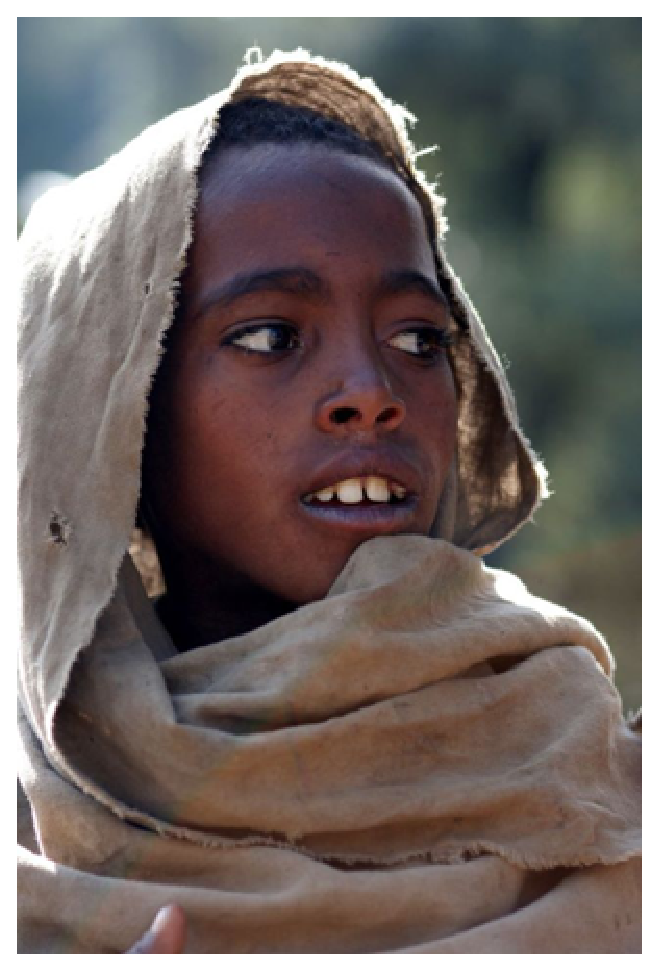
\includegraphics[scale=0.4]{etiopan.eps}
  \reflectbox{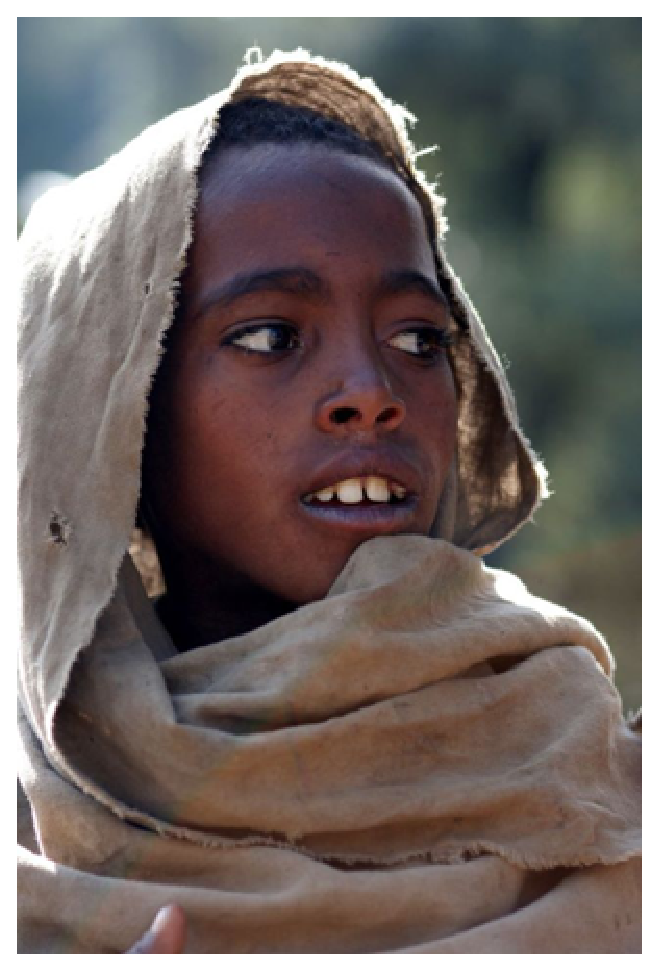
\includegraphics[scale=0.4]{etiopan.eps}}
  \caption{Malý etiopánek a jeho bratříček}
  \label{etiopan}
\end{figure}
\newpage
Rozdíl mezi vektorovým\,\dots
\begin{figure}[H]
  \centering
  
\includegraphics[width=8cm]{oniisan.eps}
  \caption{Vektorový obrázek}
  \label{vektor}
\end{figure}

\dots a bitmapovým obrázkem
\begin{figure}[H]
  \centering
  
\includegraphics[width=8cm]{oniisan2.eps}
  \caption{Bitmapový obrázek}
  \label{rastr}
\end{figure}
se projeví například při zvětšení.

Odkazy (nejen ty) na obrázky \ref{etiopan}, \ref{vektor} a \ref{rastr},
na tabulky \ref{tab:kurzy} a \ref{tab:logika} a také na algoritmus \ref{alg:fastslam}
jsou udělány pomocí křížových odkazů. Pak je ovšem potřeba zdrojový soubor přeložit dvakrát.

Vektorové obrázky lze vytvořit i přímo v \LaTeX u, například pomocí prostředí 
\texttt{picture}. Všechny rozměry jsou uváděny v mm.
\begin{figure}
  \centering
  \setlength{\unitlength}{1.3mm}
  \begin{picture}(115,158.5)

  \dashline{8}(15,0)(15,158,5)
  \dashline{8}(0,144)(115,144)

  \put(0,79.25){\vector(1,0){15}}
  \put(0,79.25){\vector(-1,0){0}}
  \put(1,81){Mezera = 15}

  \put(0,3){\vector(-1,0){0}}
  \put(0,3){\vector(1,0){115}}
  \put(50,4){Šířka stránky = 115}

  \put(112,0){\vector(0,1){158.5}}
  \put(112,0){\vector(0,-1){0}}
  \put(105,55){\vector(1,1){7}}
  \put(92,50){\minibox[c]{Výška\\ stránky = 158,5}}

  \put(90,158.5){\vector(0,-1){14.5}}
  \put(90,158.5){\vector(0,1){0}}
  \put(91,150){\minibox[c]{Výška\\ mezery = 14,5}}

  \put(90,144){\vector(0,-1){10}}
  \put(90,144){\vector(0,1){0}}
  \put(91,138){\minibox[c]{Výška\\ mezery = 10}}

  \put(90,134){\vector(0,-1){10}}
  \put(90,134){\vector(0,1){0}}
  \put(91,128){\minibox[c]{Výška\\ hlavičky = 10}}

  \put(90,124){\vector(0,-1){14}}
  \put(90,124){\vector(0,1){0}}
  \put(91,116){\minibox[c]{Výška\\ mezery = 14}}

  \put(90,110){\vector(0,-1){75}}
  \put(90,110){\vector(0,1){0}}
  \put(91,65){\minibox[c]{Výška\\ těla = 75}}

  \put(90,35){\vector(0,-1){15}}
  \put(90,35){\vector(0,1){0}}
  \put(91,27){\minibox[c]{Výška\\ mezery = 15}}

  \put(90,20){\vector(0,-1){10}}
  \put(90,20){\vector(0,1){0}}
  \put(91,14){\minibox[c]{Výška\\ paty = 10}}

  \put(30,137){\vector(1,0){55}}
  \put(30,137){\vector(-1,0){0}}
  \put(50,138){Šířka boxu = 55}

  \put(85,87){\vector(1,0){9}}
  \put(85,87){\vector(-1,0){0}}
  \put(94,87){\vector(1,0){15}}
  \put(94,87){\vector(-1,0){0}}
  \put(95,90){\minibox[c]{Šířka\\ boxu = 15}}
  \put(94,97){\vector(-1,-3){3.3}}
  \put(91,98){Mezera = 9}

  \thicklines
  \put(0,0){\framebox(115,158.5)}
  \put(30,124){\framebox(55,10){\bf{Hlavička}}}
  \put(30,35){\framebox(55,75){\bf{Textové tělo}}}
  \put(94,74.25){\framebox(15,10){\bf{\minibox[c]{Okrajová\\ poznámka}}}}
  \put(30,10){\framebox(55,10){\bf{Pata}}}
  \end{picture}
  \caption{Vektorový obrázek v prostředí \texttt{picture}}
\end{figure}
\end{document}
